\section{The Identity-Transformation Framework}
%\section{The Identifier-Transformation Approach of UPPRESSO}
\label{sec:challenge}

This section investigates the security requirements of privacy-preserving SSO,
    and explains the identity dilemma.
Then,
    we present the identity-transformation framework.


\subsection{Security Requirements of SSO}
\label{subsec:basicrequirements}
%A dedicated, the bidirectional authenticated secure channel was proposed to improve the confidentiality and integrity of identity token \cite{CaoSBKVC14}.

The primary goal of non-anonymous SSO services is %user authentication and identification \cite{SPRESSO},
 to ensure that a \emph{legitimate} user is able to login to an \emph{honest} RP as his permanent account at this RP, %correlating multiple login instances,
    by presenting the \emph{identity tokens} issued by the \emph{honest} IdP.

To achieve this goal,
 an identity token generated by the IdP \cite{OpenIDConnect,rfc6749,SAML,SAMLIdentifier,NIST2017draft,BrowserID,SPRESSO} specifies (\emph{a}) the RP to which the user requests to login (i.e., \emph{RP designation})
    and  (\emph{b}) the user who is authenticated by the IdP (i.e., \emph{user identification}).
Therefore,
    an honest RP compares the designated RP identity (or pseudo-identity) in identity tokens with its own before accepting the tokens;
     otherwise,
        a malicious RP could replay a received identity token to the honest RP and login as the victim user.
The RP allows the token holder to login as the user (pseudo-)identity specified in the accepted tokens.

The SSO login flow also requires \emph{confidentiality} and \emph{integrity} of identity tokens.
An identity token should be forwarded by the authenticated user to the target RP only,
    not leaked to any other parties;
        otherwise, an adversary who presents the token, would successfully login to the RP.
Integrity is necessary
    to prevent adversaries from tampering with a token.
So identity tokens are signed by the IdP and usually transmitted over HTTPS \cite{OpenIDConnect,rfc6749,SAML}.

These security requirements (i.e., RP designation, user identification, confidentiality, and integrity) of SSO identity tokens
     are well discussed \cite{ArmandoCCCT08,FettKS16, FettKS17},
     and
     vulnerabilities breaking any of the properties
            result in attacks \cite{SomorovskyMSKJ12, WangCW12, ArmandoCCCPS13, ZhouE14, WangZLLYLG15, WangZLG16, YangLLZH16, MainkaMS16, MainkaMSW17, YangLCZ18, YangLS17, ShiWL19, ChenPCTKT14, ccsSunB12, DiscoveringJCS, dimvaLiM16, CaoSBKVC14, TowardsShehabM14}.
%An adversary might attempt to login to an honest RP as a victim user (i.e., \emph{impersonation}),
% or allure a victim user to login to an honest RP as the attacker (i.e.,  \emph{identity injection}).
%Friendcaster used to accept any received identity token, which violates RP designation \cite{ChenPCTKT14},
%    so a malicious RP could replay a received identity token to Friendcaster and login as the victim user.
%The defective IdP of Google ID SSO signs identity tokens where the Email element was not enclosed,
%        while some RPs use a user's Email as his unique username \cite{WangCW12}.
%So this violation of user identity resulted in vulnerable services.
%Because identity tokens were leaked in different ways \cite{WangCW12,ccsSunB12,ArmandoCCCPS13,DiscoveringJCS,dimvaLiM16},
% the eavesdroppers could impersonate the victim users.
%Some RPs even accept user attributes that are not bound in identity tokens (i.e., a violation of integrity) \cite{WangCW12},
%  so that adversaries could insert arbitrary attributes into the identity tokens to impersonate another user at these RPs.




\subsection{The Identity Dilemma of Privacy-Preserving SSO}
\label{subsec:challenges}
\begin{table}[t]
\footnotesize
    \caption{The (pseudo-)identities in privacy-preserving SSO.}
    \centering
%    \begin{tabular}{|l|l|l|}
    \begin{tabular}{|p{1.0cm}|p{5.1cm}|p{1.13cm}|} \hline
    {\textbf{Notation}} & {\textbf{Description}} & {\textbf{Lifecycle}} \\ \hline
    {$ID_U$} & {The user's unique identity at the IdP.} & {Permanent} \\ \hline
    {$ID_{RP_j}$} & {The $j$-th RP's unique identity at the IdP.} & {Permanent} \\ \hline
    {$PID_{U,j}^i$} & {The user's pseudo-identity, in the user's $i$-th login instance to the $j$-th RP.} & {Ephemeral} \\ \hline
    {$PID_{RP_j}^i$} & {The $j$-th RP's pseudo-identity, in the user's $i$-th login instance to this RP.} & {Ephemeral} \\ \hline
    {$Acct_j$} & {The user's identity (or account) at the $j$-th RP.} & {Permanent} \\ \hline
    \end{tabular}
    \label{tbl:notations-dilemma}
\end{table}


We aim to design a privacy-preserving SSO system with the four security properties as above,
    while preventing the privacy threats due to both the IdP-based login tracing and the RP-based identity linkage.
Table \ref{tbl:notations-dilemma} lists the notations in the following explanations,
    and the subscript $j$ and/or the superscript $i$ may be omitted when there is no ambiguity.
We explicitly distinguish a user's identity (or \emph{account}) at the RP, 
     from the user's \emph{identity} at the IdP and the user's \emph{pseudo-identity} enclosed in identity tokens.

An identity token contains the (pseudo-)identities of the authenticated user and the target RP. %which is to tell the RP that this user has been authenticated by the IdP.
% Let us denote the long-term unique identifiers of the user and the RP as $ID_U$ and $ID_{RP}$, respectively.
Since the IdP authenticates users and always knows the user's identity (i.e., $ID_U$),
    to prevent the IdP-based login tracing,
    we shall not reveal the target RP's permanent identity (i.e., $ID_{RP}$) to the IdP.
So an \emph{ephemeral} pseudo-identity for the RP (i.e., $PID_{RP}$) shall be used in the identity-token request:
(\emph{a}) to ensure RP designation,
     $PID_{RP}$ shall be \emph{uniquely} associated with the target RP;
    and (\emph{b}) the IdP cannot derive any information about $ID_{RP}$ from any $PID_{RP}^i$,
        which implies $PID_{RP}^i$ in multiple login instances shall
         be independent of each other.\footnote{Even when the target RP is kept unknown to the IdP,
            the IdP shall not link multiple login instances visiting this RP.}
   % the IdP-based login tracing is still effective, to correlate a user's multiple login instances.

To prevent the RP-based identity linkage,
 the IdP does not enclose $ID_U$ in identity tokens.
A user pseudo-identity (i.e., $PID_U$) is bound instead:
    (\emph{a}) in multiple login instances to an RP, $PID_U^i$ shall be independent of each other and generated ephemerally,
        to prevent the IdP-based login tracing;\footnote{If $PID_U^i$ is not completely independent of each other,
         it implies the IdP could link multiple login instances visiting this RP.}
    (\emph{b}) the RP cannot derive any information about $ID_U$ from any $PID_{U,j}$,
    which implies $PID_{U,j}$ for different RPs shall be independent of each other;
    and (\emph{c}) to ensure user identification,
    an \emph{ephemeral} $PID_{U}^i$ in each login instance shall enable the RP to correlate it
     with the \emph{permanent} account  (i.e., $Acct$) at this RP.


Given a user,
    (\emph{a}) an identity token contains only pseudo-identities, i.e., $PID_{U,j}^i$ and $PID_{RP_j}^i$,
        which are independent of each other for different RPs and in multiple login instances, respectively,
    and (\emph{b}) the two \emph{ephemeral} pseudo-identities enable the target RP to derive a \emph{permanent} account, i.e., $Acct_j$.
The relationship among the (pseudo-)identities in identity tokens is illustrated in Figure \ref{fig:IDCorrelation}.
The \emph{red} and \emph{green} blocks represent \emph{permanent} and \emph{ephemeral} (pseudo-)identities, respectively.
The arrows denote the transformations of (pseudo-)identities.
%It describes the {\em identity dilemma} of privacy-preserving SSO as below:


\begin{figure}[bt]
  \centering
  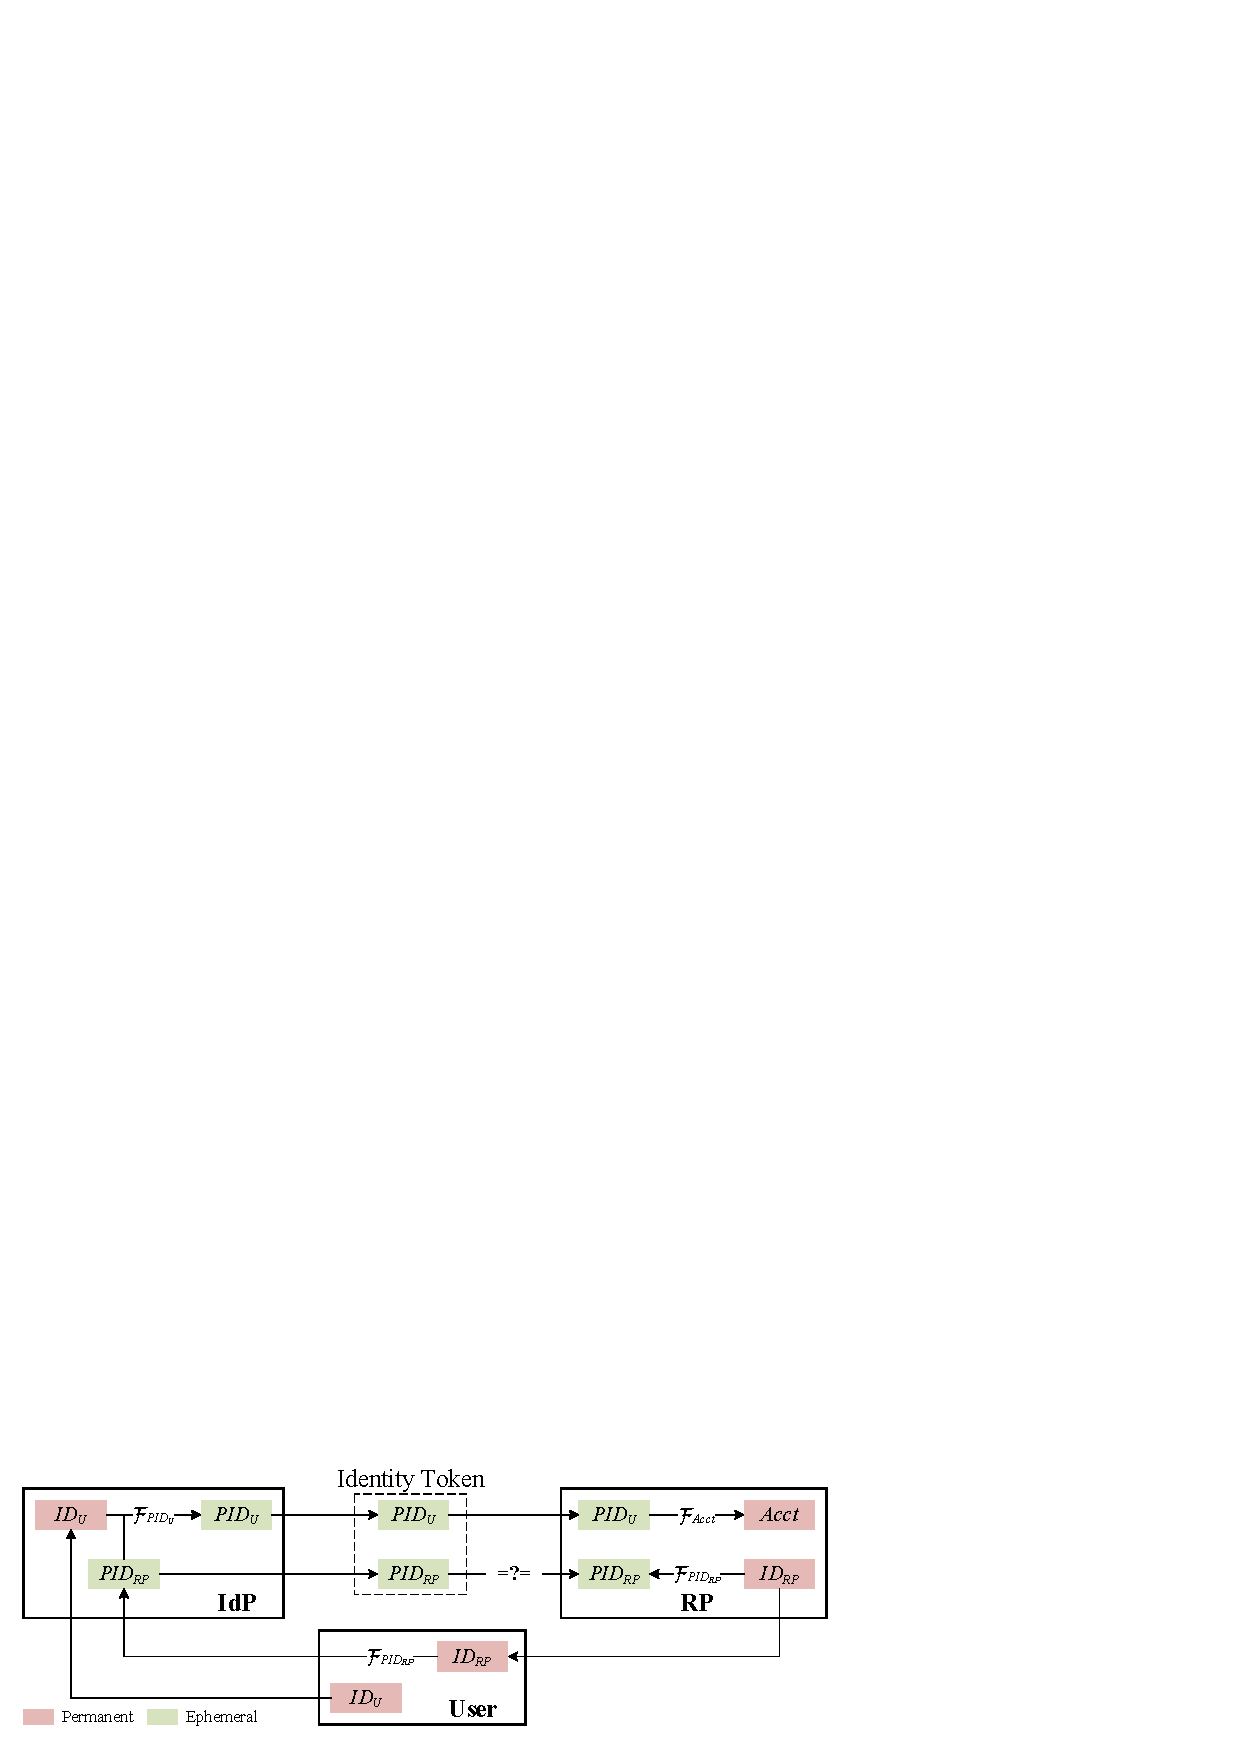
\includegraphics[width=0.98\linewidth]{fig/IDCorrelation.pdf}
  \caption{Identity transformations in privacy-preserving SSO.}
  \label{fig:IDCorrelation}
\end{figure}

To satisfy the requirements of both security and privacy,
     we pose the following \emph{identity dilemma} of SSO identity tokens:

\noindent\emph{Given an authenticated user and an unknown RP (i.e., permanent $ID_U$ and ephemeral $PID_{RP}$),
    the IdP is expected to generate an ephemeral pseudo-identity (i.e., $PID_{U}$)
     which will be correlated with the user's permanent identity at this RP (i.e., $Acct$),
     while knowing nothing about the RP's identity or the user's account at this RP (i.e., $ID_{RP}$ or $Acct$).}

Existing privacy-preserving SSO solutions (i.e., SPRESSO \cite{SPRESSO}, BrowserID \cite{BrowserID} and PPID \cite{NIST2017draft})
  do not explicitly and comprehensively consider all five (pseudo-)identities in the SSO login flow,
    and either $ID_U$ or $ID_{RP}$ is still enclosed in identity tokens.


\subsection{Identity Transformation}
\label{subsec:solutions}

%In the identity dilemma, we explicitly separate a user's account at the RP
%     from the user's unique identity at the IdP and the user's  pseudo-identity in identity tokens.
%This method guides us to propose the identity-transformation framework
%    (and then to solve the identity dilemma).


%we should provide the IdP some information related to the user's $Account$ at the RP to assist the generation of $PID_U$,
% so that $PID_U$ can be correctly correlated with the $Account$. Meanwhile, such information should not provide any additional knowledge for the IdP to derive the RP's identity, or for two RPs to correlate two $Account$s belonging to the same user.
The privacy protection of SSO is converted into a challenge
 to design \emph{identity-transformation functions} as below.
\vspace{-\topsep}\begin{itemize}
\setlength{\topsep}{0pt}
\setlength{\partopsep}{0pt}
\setlength{\itemsep}{0pt}
\setlength{\parsep}{0pt}
\setlength{\parskip}{0pt}
\item
$\mathcal{F}_{PID_{RP}}(ID_{RP}) = PID_{RP}$, calculated by the user and the RP.
From the IdP's view,
$\mathcal{F}_{PID_{RP}}()$ is a one-way function and $PID_{RP}$
is indistinguishable from random variables.
\item
$\mathcal{F}_{PID_U}(ID_U, PID_{RP}) = PID_{U}$, calculated by the IdP.
From the RP's view,
    $\mathcal{F}_{PID_U}()$ is a one-way function and $PID_{U}$ is indistinguishable from random variables.
\item
$\mathcal{F}_{Acct}(PID_{U}, PID_{RP}) = Acct$, calculated by the RP.
Given $ID_U$ and $ID_{RP}$, $Acct$ keeps permanent and unique to other accounts at this RP.
In the user's any $i$-th and $i'$-th ($i \neq i'$) login instances to the RP,
 $\mathcal{F}_{Acct}(PID_{U}^i, PID_{RP}^i) = \mathcal{F}_{Acct}(PID_{U}^{i'}, PID_{RP}^{i'})$.
\end{itemize}

In an SSO login flow with identity transformations,
    a user firstly negotiates an ephemeral $PID_{RP}$ with the target RP.
An identity-token request with $PID_{RP}$ is sent by the user to the IdP.
After authenticating the user as $ID_U$, the IdP calculates an ephemeral $PID_U$ based on $ID_U$ and $PID_{RP}$,
    and issues an identity token binding $PID_U$ and $PID_{RP}$.
%It is forwarded by the user to the RP.
After matching the designated RP pseudo-identity in the token,
    the RP calculates $Acct$ and allows the token holder to login as $Acct$.

%The identity-transformation functions satisfy the privacy requirements,
%    while the authentication and authorization between users and the IdP is still kept independent of the steps involving identity tokens.

%After identity transformations are adopted,
%    the steps dealing with identity tokens work compatibly with any type of user credentials
%        and independently of the user-attribute authorizations,
%        as those in the commonly-used SSO protocols \cite{OpenIDConnect,rfc6749,SAML,NIST2017draft}.

